%! TEX root = main.tex

\section{Solución}

Se diseña y desarrolla un Juego Serio para dispositivos móviles llamado
\textit{eTesai}, el cual consiste ofrece a los  estudiantes de enfermería un
medio para realizar procedimientos de enfermería y cuyo objetivo es servir como
herramienta de apoyo en el aprendizaje.

\subsection{Arquitectura}

En la figura~\ref{fig:full_architecture} se observa los componentes de la
solución, y las herramientas utilizadas para su desarrollo.

\begin{figure}[H]
\centering
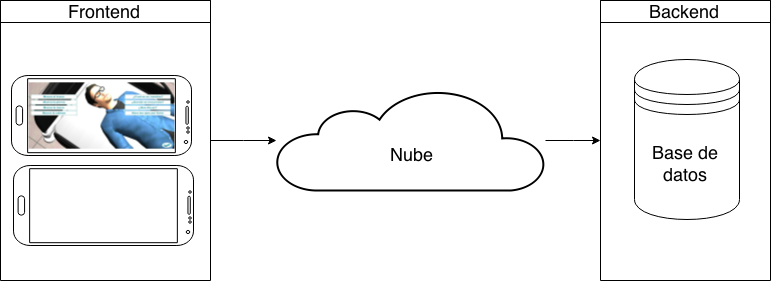
\includegraphics[scale=0.29]{images/full.png}
\caption{Esquema general de componentes de \textit{eTesai}}
\label{fig:full_architecture}
\end{figure}

La solución se compone de un \textit{FrontEnd} que es una aplicación
\textit{Android}, la cual es utilizada por los estudiantes de enfermería. Los
registros de uso del \textit{FrontEnd} son almacenados bajo demanda en un
servidor \textit{BackEnd}, el cual se encarga de asociar los registros con los
alumnos y almacenarlos de manera persistente.


\subsection{Tecnologías utilizadas}

El motor de videojuegos utilizado para el desarrollo de \textit{eTesai} es
\textit{Unity3D}, en su versión gratuita. \textit{Unity3D} es desarrollado por
\textit{Unity Technologies} y posee un motor de \textit{renderizado}, un flujo
de trabajo para la creación de contenido 3D interactivo, y permite mezclar
contenido 3D, 2D, sonidos y animaciones en un entorno de desarrollo integrado.
\textit{Unity3D} permite desarrollar aplicaciones para múltiples sistemas
operativos, como \textit{Android, iOs, Windows Phone}, entre
otros\cite{unity3d}.

% Agregar referencias
El \textit{Backend} es desarrollado utilizando \textit{Java EE 7}, servicios web
\textit{REST}, y \textit{Eclipse} como entorno de desarrollo integrado. El
código fuente del \textit{FrontEnd} es desarrollado con \textit{MonoDevelop}.

\subsection{Hipótesis asumidas}

Existen acciones que requieren de un esfuerzo significativo para ser simuladas,
por ello. Estas acciones deben formar parte del procedimiento, pero el nivel de
detalle simulado no es importante, por ello se formulan hipótesis sobre estos
que permiten guiar la simulación de los mismos.

Estas hipótesis son:

\begin{itemize}
\item 
    \textbf{Comandos de voz con interfaz}:  para enviar una petición o informarle 
    sobre algo al paciente (por ejemplo, dar detalles del procedimiento), 
    no es necesario identificar las palabras del usuario, sino más bien detectar
    que ha hablado y listar las posibles acciones que se pueden realizar.
    
\item \textbf{Extracción uniforme de elementos}: para realizar la acción de
    extraer un elemento utilizado en el paciente, se considera que realizarlo de
    una sola manera para todos los elementos convierte a la interfaz más
    intuitiva.

\item \textbf{Acciones por interfaz de usuario}: acciones que se realizan
    directamente sobre el paciente (sin la utilización de elementos), son
    complejas de simular, es suficiente con una opción en la interfaz que
    permita al usuario realizarlas. 
    
\item \textbf{Acciones de bioseguridad}: la bioseguridad, que es un aspecto
    fundamental y transversal a todo procedimiento de enfermería. Se considera
    suficiente que el estudiante sepa el momento en el que deba realizar
    acciones relacionadas con la bioseguridad.
    
\item \textbf{Representación iconográfica}: para representar el estado del
    enfermero es suficiente mostrar una imagen representativa. Es decir, que
    para mostrar que el enfermero tiene una gorra, es suficiente mostrar una
    imagen de una gorra. Esta hipótesis se aplica para las opciones de
    bioseguridad, las opciones para la utilización de elementos así como para la
    representación del elemento seleccionado.

\item \textbf{Factores motivantes}: indicadores de rendimiento, como un puntaje
    al final de cada procedimiento, y el tiempo total dentro del procedimiento,
    impactan positivamente en el involucramiento del usuario. La interacción
    social es otro factor que incrementa el nivel de compromiso del usuario.

\item \textbf{Falta de pistas}: la ausencia de signos visuales que indiquen las
    acciones que debe realizar el usuario durante la experiencia, permite al
    usuario probar sus conocimientos, e impide al usuario avanzar en el
    procedimiento utilizando una técnica de \emph{prueba y error}.

\end{itemize}

\subsection{Frontend}

El \textit{FrontEnd} es una aplicación \textit{Android}, con un flujo que se observa en la
figura~\ref{fig:flujo_frontend}, la misma se inicia en la escena \emph{Inicio},
que permite al usuario seleccionar varias opciones y navegar a las demás
escenas.

\begin{figure}[H]
\centering
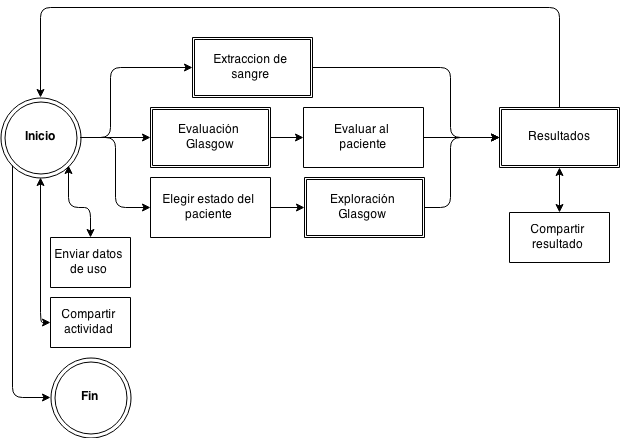
\includegraphics[scale=0.29]{../solucion/images/grafo_escenas.png}
\caption{Flujo de pantallas de la solución}
\label{fig:flujo_frontend}
\end{figure}

En las escenas, el usuario tiene dos formas de interactuar con el punto de
vista, la solución permite \textit{a)} alejar o acercar la cámara, y,
\textit{b)} mover la cámara alrededor del paciente.

Las acciones realizadas por los usuarios, así como el resultado de sus acciones,
son registradas en el dispositivo del usuario, y luego es enviada a un servidor
para su persistencia.

\subsection{Backend}

La solución almacena información detallada acerca de las acciones del usuario,
las condiciones de estas acciones y el contexto en el cual fueron ejecutadas.

Esta información es almacenada en un servidor dedicado para su posterior
análisis.

La información almacenada en el servidor permite reproducir completamente la
sesión de juego de un usuario, esta información es interesante para analizar los
puntos débiles y fuertes de los usuarios y de la solución.

\subsection{Escenas}

La solución presenta procedimientos de enfermería en forma de escenas simuladas.
Los procedimientos son seleccionados en conjunto con profesionales del área de
enfermería del \gls{iab}. 

El procedimiento de extracción de muestras sangre, es representada dentro de la
solución en la escena \emph{Extracción de muestras Sangre}. El procedimiento de
evaluación de un paciente utilizando la escala de \textit{Glasgow}, es
representado en la escena \emph{Glasgow}.

\subsection{Extracción de muestras sangre}

En la figura~\ref{fig:hemocultivo_principal} se observa el inicio de la escena
\emph{Extracción de muestras de sangre}, el objetivo principal de este
procedimiento es extraer muestras de la sangre del paciente para su análisis en
un laboratorio. El procedimiento formal, según los profesores del
\gls{iab} y~\cite{oms:extraccion}, cuenta con $22$ pasos.

\begin{figure}[H] 
\centering 
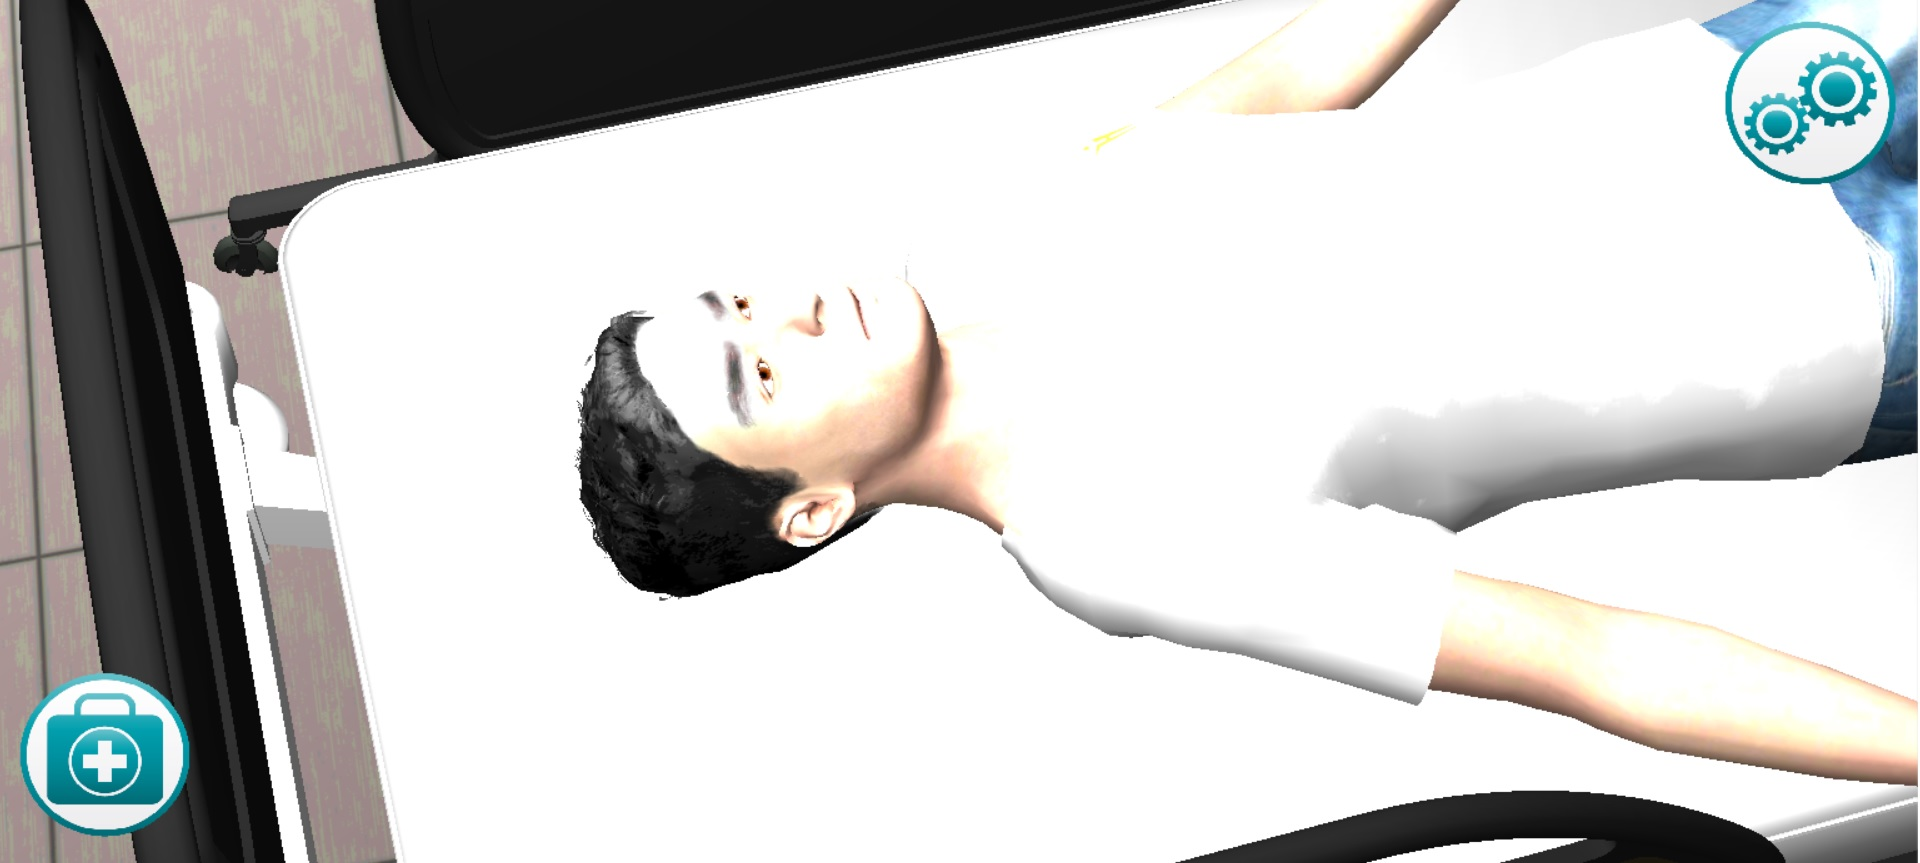
\includegraphics[width=8cm]{../solucion/images/hemocultivo_principal.jpg}
\caption{Pantalla principal de la escena \emph{Extracción de muestras extracción
        de sangre}.}
\label{fig:hemocultivo_principal}
\end{figure}

En este procedimiento, el usuario interactúa con varios objetos que son
necesarios para llevar a cabo el procedimiento, en la
figura~\ref{fig:hemocultivo_jeringa_zoom} se observa la jeringa en el brazo del
paciente, con flechas ilustrativas que muestran como mover los dedos para
realizar la extracción de la sangre.

\begin{figure}[H]
\centering 
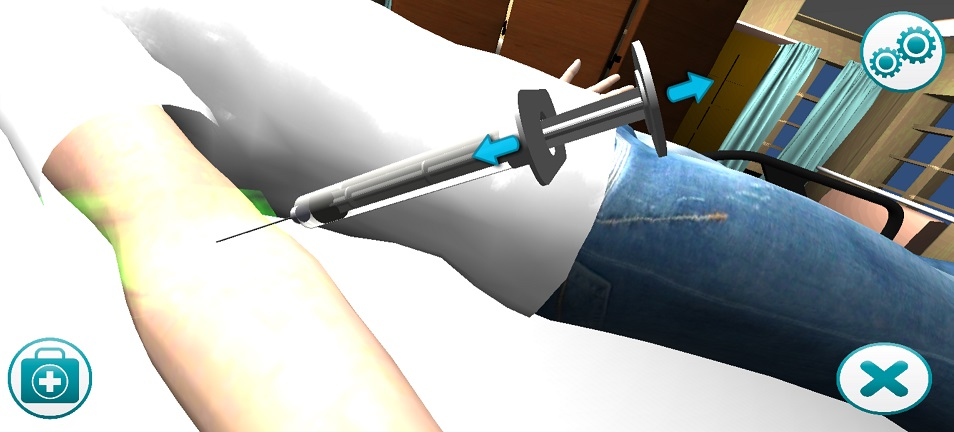
\includegraphics[width=8cm]{../solucion/images/hemocultivo_jeringa_ampliada.jpg}
\caption{Vista de la jeringa ampliada, facilitando la extracción de sangre.}
\label{fig:hemocultivo_jeringa_zoom}
\end{figure}

En la figura~\ref{fig:hemocultivo_gui} se observa la interfaz gráfica, con
opciones de bioseguridad y de utilización de elementos.

\begin{figure}[H]
\centering
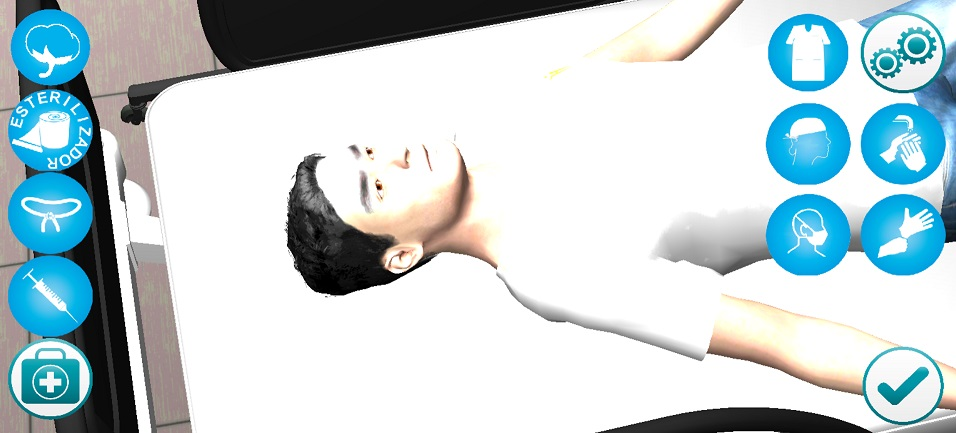
\includegraphics[width=8cm]{../solucion/images/hemocultivo_gui.jpg}
\caption{Escena \emph{Extracción de Sangre}}
\label{fig:hemocultivo_gui}
\end{figure}

Durante el procedimiento se utiliza un motor de reglas condicionado por
eventos\cite{bailey2004event,behrends2006combining}, este motor permite
reaccionar ante las acciones del usuario y verificar el cumplimiento de los
pasos del procedimiento. 

\begin{figure}[H]
\centering 
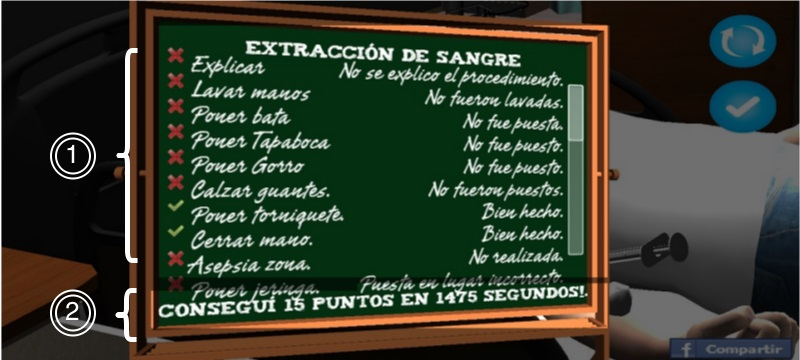
\includegraphics[width=8cm]{../solucion/images/hemocultivo_retroalimentacion.jpg}
\caption{Retroalimentación y puntuación final de la escena \emph{Extracción de
        sangre}.}
\label{fig:hemocultivo_retroalimentacion}
\end{figure}

En la parte $1$ de la figura~\ref{fig:hemocultivo_retroalimentacion}, se puede
ver como se brinda información al  usuario acerca de su rendimiento. Esta
información le indica los pasos que realizó de manera correcta o incorrecta y
las razones por las cuales tuvo ese desempeño.

Cada regla tiene asociado un peso, de acuerdo a la dificultad de realizar el
paso, este peso es utilizado al final de la partida para dar una puntuación al
usuario como se muestra en el punto $2$ de la
figura~\ref{fig:hemocultivo_retroalimentacion}. Junto al puntaje final también
se muestra el tiempo que le tomó al usuario completar el procedimiento.

\subsection{Glasgow}

La escena \emph{Valoración de la escala de Glasgow}, cuya interfaz principal se
observa en la figura~\ref{fig:glasgow_principal}, el objetivo principal de esta
escena es diagnosticar el estado de conciencia de un paciente en estado crítico,
utilizando la escala de \textit{Glasgow}\cite{protocolo}. 

\begin{figure}[H]
\centering
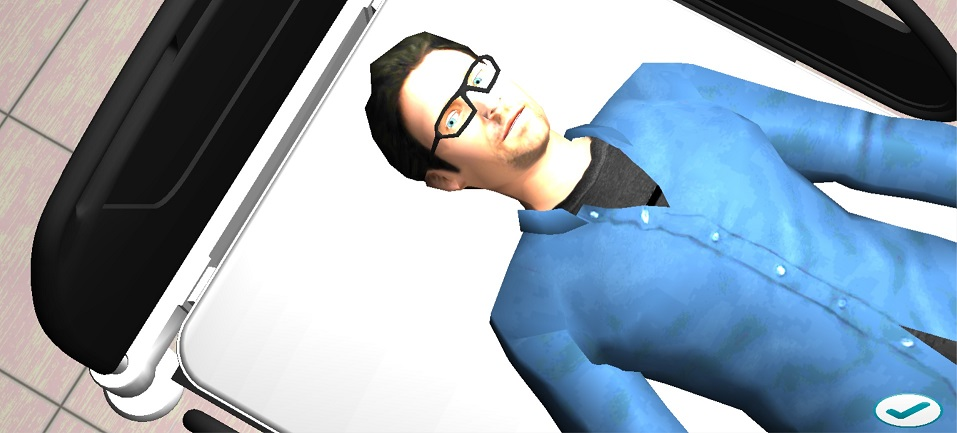
\includegraphics[width=8cm]{../solucion/images/glasgow_principal.jpg}
\caption{Interfaz de la escena de \emph{Valoración de la escala de Glasgow.}}
\label{fig:glasgow_principal}
\end{figure}

Esta escena tiene dos versiones. La primera versión, denominada
\emph{Evaluación}, se inicia con un paciente en un estado aleatorio, y la tarea
el alumno es descubrir el estado del paciente. En la segunda versión, denominada
\emph{Exploración}, el usuario elige el estado inicial del paciente, y sirve
para que el mismo observe como reacciona un paciente con un diagnostico dado.

El protocolo indica que el enfermero debe analizar tres aspectos del paciente,
la visión (del $1$ al $4$), la audición (del $1$ al $5$) y la capacidad motora
(del $1$ al $6$)\cite{protocolo}. Realizada la valoración del
paciente, el enfermero debe sumar los puntajes obtenidos, y así realizar un
diagnostico, de $13$ a $15$ el daño es leve, de $9$ a $12$ el daño es moderado y
de $3$ a $8$ el daño es severo\cite{helmick2007mild}.


\begin{figure}[H]
\centering
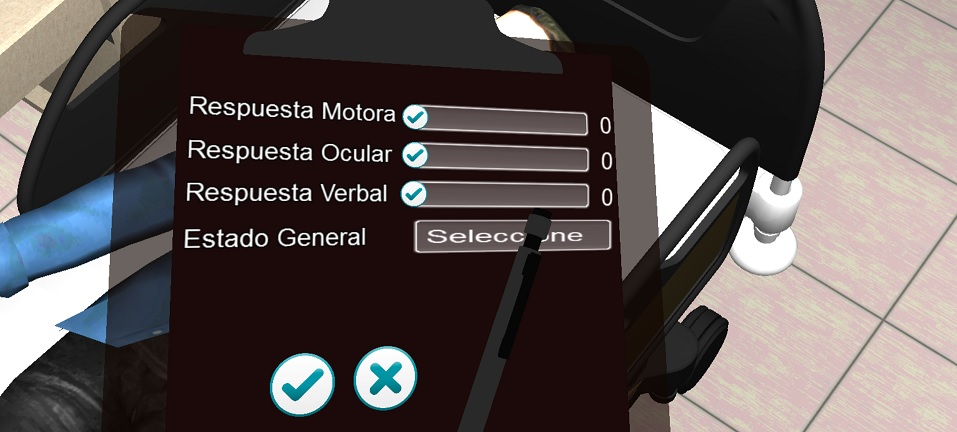
\includegraphics[width=8cm]{../solucion/images/glasgow_diagnostico.jpg}
\caption{Vista de la \emph{Pantalla de diagnóstico}.}
\label{fig:glasgow_gui_resultados}
\end{figure}

El diagnostico del usuario es contrastado con el estado real del paciente, para
mostrar el resultado de la escena, en la figura~\ref{fig:glasgow_resultado}
marcado por el $1$ se observa la retroalimentación dada al usuario.

Para el cálculo del puntaje final que se le mostrará al usuario, por cada
respuesta dada en la \emph{Pantalla de diagnóstico} se asigna una puntuación de
acuerdo a que tan cerca estuvo el usuario de la respuesta correcta. Se suman
estos valores y se calcula el porcentaje de acierto. El puntaje final junto a el
tiempo que tardó el usuario realizando el procedimiento son presentados como se
observa en la figura~\ref{fig:glasgow_resultado} marcado por el $2$.

\begin{figure}[H]
\centering
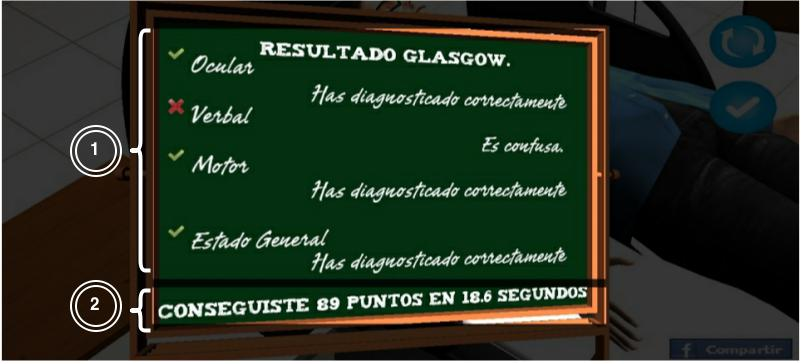
\includegraphics[width=8cm]{../solucion/images/glasgow_resultado.jpg}
\caption{Retroalimentación y puntuación final de la escena \emph{Glasgow}.}
\label{fig:glasgow_resultado}
\end{figure}
